%% Autor: Björn Ritterbecks 
%% Letzte Aenderung: 15.06.2016 
\thisfloatsetup{%
  capbesidewidth=\marginparwidth}
\begin{figure}[htbp]
\centering
%\sansmath
 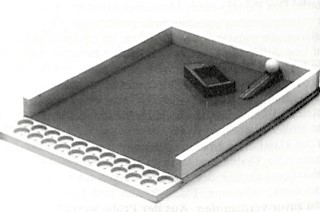
\includegraphics[width=0.99\textwidth]{images/graf.jpg}
  \caption[Funktionsmodell eines Massenspektrometers von Bühler und Graf]{Funktionsmodell eines Massenspektrometers von Bühler und Graf. Tischtennisbälle werden durch eine kleine Bohrung mit Eisenwolle und/oder Nylonwatte befüllt, um Masse-Ladungs-Verhältnisse nachzuahmen (entnommen aus \cite[S\,34]{Graf2002}).}
  \label{fig:graf}
  \vspace{-0pt}
\end{figure}